\section{Quantum communication systems with PASSs}
    The use of squeezed states instead of coherent states allows us to overcome the limits
    of PACSs. The representation of a noisy squeezed state $\Operator{\varXi}_{\mathrm{th}}(\mu,\zeta)$ is given in 
    \ref{squeezedStates} and the performance analysis without thermal noise is given in 
    \ref{SS_performance}.
    The noisy PASSs $\Operator{\varXi}_{\mathrm{th}}^{(k)}(\mu,\zeta)$ correspondent to the squeezed state
    $\Operator{\varXi}_{\mathrm{th}}(\mu,\zeta)$ is obtained using the equation
    \ref{eq:photonAddedState}, as it is described in \ref{PASSs}. This section discusses the advantages of using PASSs 
    in quantum OOK and BPSK systems.

    The MDEP for PASSs systems is found again with the Helstrom bound \ref{eq:HelstromBound}.
    As for the other systems, it is useful to define the mean number of photons $n_p$ for noisy 
    photon added squeezed states, that is given by:
    \begin{equation}
        n_p(\mu,\zeta,\bar{n}) = \frac{N_{k+1}(\mu,\zeta,\bar{n})}{N_k(\mu,\zeta,\bar{n})}-1,
        \label{eq:np_PASS}
    \end{equation}
    where
    \begin{equation}
        \begin{split}
            N_k(\mu,\zeta,\bar{n}) &= \tr{(\Operator{A}^\dagger)^k \Operator{\varXi}_{\mathrm{th}}(\mu,\zeta) \Operator{A}^k}\\
                                    &= \tr{(\Operator{A}^\dagger)^k \Operator{D}_\mu \Operator{S}_\zeta \Operator{\varXi}_{\mathrm{th}}
                                    \Operator{S}_\zeta^\dagger \Operator{D}_\mu^\dagger \Operator{A}^k}.
        \end{split}
    \end{equation}

    \subsection{Quantum OOK}
        The constellation of a quantum OOK system with noisy PASS, is given by:
        \begin{subequations}
            \begin{align}
                \Operator{\varXi}_0 &= \Operator{\varXi}_{\mathrm{th}}^{(0)}(0,0)\\
                \Operator{\varXi}_1 &= \Operator{\varXi}_{\mathrm{th}}^{(k)}(\mu,\zeta).
            \end{align}
        \end{subequations}
        In figure \ref{fig:3.6}, the MDEP of a quantum OOK noisy PASS system is plotted in function
        of the mean number of photon $\bar{n}_p$ in the system. For the simulation are used $N=30$, $\bar{n}=10^{-2}$, $\theta=\pi$ and
        equiprobable symbols.
        It can be noticed that the photon addition significantly improves the performance of the system,
        at least for the plotted energy level.

    \subsection{Quantum BPSK}
        Similary to the PACS BPSK, the constellation of PASS BPSK is given by:
        \begin{subequations}
            \begin{align}
                \Operator{\varXi}_0 &= \Operator{\varXi}_{\mathrm{th}}^{(k)}(-\mu,\zeta)\\
                \Operator{\varXi}_1 &= \Operator{\varXi}_{\mathrm{th}}^{(k)}(\mu,\zeta).
            \end{align}
        \end{subequations}
        
        The figure \ref{fig:3.7} shows the effects of the photon addition in a quantum BPSK
        system, in terms of the mean photon number in the system $\bar{n}_p$, given by the average of 
        the mean photon number $n_p$ of $\Operator{\varXi}_0$ and $\Operator{\varXi}_1$. The parameters used
        for the simulation are $N=40$, $\bar{n}=10^{-2}$, $\theta=\pi$ and equiprobable symbols.
        As in PACS case, it is evident that the photon addition, in a BPSK system, has not
        the positive effect that has in an OOK system.
        
        \begin{figure}[t]
            \begin{center}
                %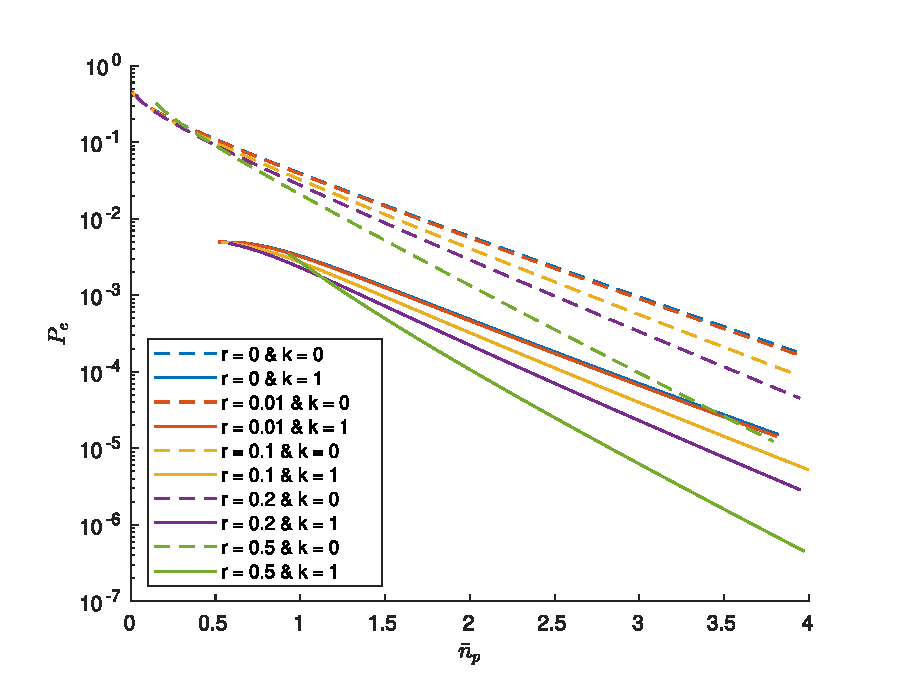
\includegraphics[width=0.8\textwidth]{fig3.6.eps}
                % This file was created by matlab2tikz.
%
%The latest updates can be retrieved from
%  http://www.mathworks.com/matlabcentral/fileexchange/22022-matlab2tikz-matlab2tikz
%where you can also make suggestions and rate matlab2tikz.
%
\definecolor{mycolor1}{rgb}{0.00000,0.44706,0.74118}%
\definecolor{mycolor2}{rgb}{0.85098,0.32549,0.09804}%
\definecolor{mycolor3}{rgb}{0.92941,0.69020,0.12941}%
\definecolor{mycolor4}{rgb}{0.49020,0.18039,0.56078}%
\definecolor{mycolor5}{rgb}{0.46667,0.67451,0.18824}%
%
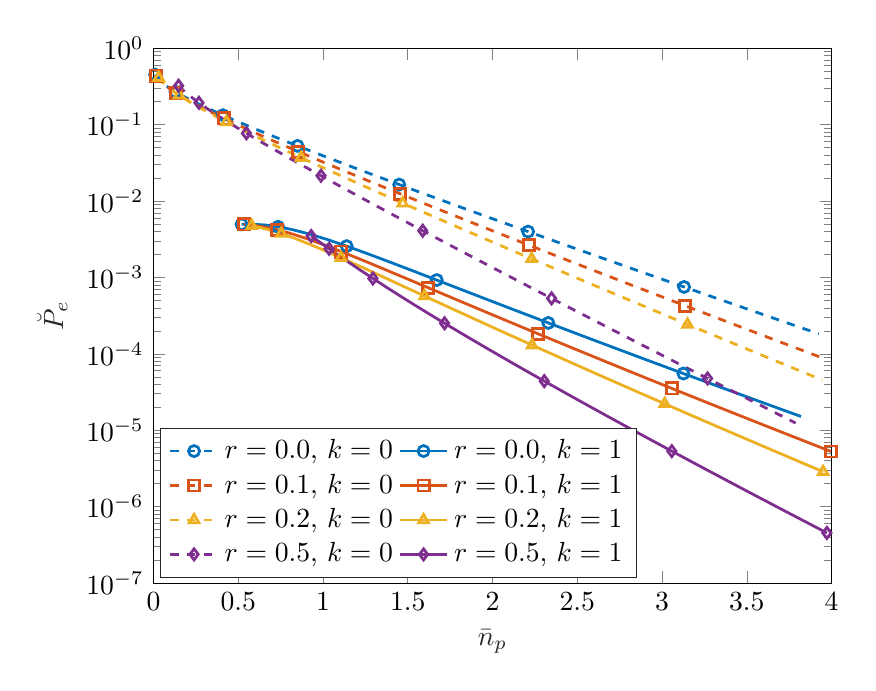
\begin{tikzpicture}

\begin{axis}[%
width=4.521in*0.75,
height=3.566in*0.75,
at={(0.758in,0.481in)},
scale only axis,
xmin=0,
xmax=4,
xlabel style={font=\color{white!15!black}},
xlabel={$\bar{n}_p$},
ymode=log,
ymin=1e-07,
ymax=1,
yminorticks=true,
ylabel style={font=\color{white!15!black}},
ylabel={$\breve{P}_e$},
axis background/.style={fill=white},
%axis x line*=bottom,
%axis y line*=left,
legend style={at={(0.01,0.01)}, anchor=south west, legend cell align=left, align=left, draw=white!15!black, legend columns=2}
]
\addplot [color=mycolor1, dashed, line width=1.0pt, mark=o, mark options={solid, mycolor1}, mark repeat={4}]
  table[row sep=crcr]{%
%0.0100000000010203	0.5\\
0.0100000000005099	0.451090572691058\\
0.0250000000005101	0.402886691283792\\
0.0500000000005101	0.356065452094155\\
0.08500000000051	0.311248795396144\\
0.13000000000051	0.268980151318818\\
0.18500000000051	0.229705791588748\\
0.25000000000051	0.193761885698297\\
0.32500000000051	0.161367836859558\\
0.41000000000051	0.132626017381623\\
0.50500000000051	0.107527572164159\\
0.61000000000051	0.0859635483991091\\
0.72500000000051	0.0677402706067526\\
0.850000000000511	0.0525976380078704\\
0.98500000000051	0.0402288938163128\\
1.13000000000051	0.030300412747497\\
1.28500000000051	0.0224701735043473\\
1.45000000000051	0.0164038154402497\\
1.62500000000051	0.0117874985937506\\
1.81000000000051	0.00833715723539569\\
2.00500000000051	0.00580411358757593\\
2.21000000000051	0.00397735316445369\\
2.42500000000051	0.00268301603344667\\
2.65000000000051	0.00178180465531275\\
2.88500000000051	0.00116504474732931\\
3.13000000000051	0.000750076554437373\\
3.38500000000051	0.000475529564681665\\
3.65000000000051	0.000296878649024612\\
3.92500000000051	0.000182524960914532\\
};
\addlegendentry{$r = 0.0$, $k = 0$}

\addplot [color=mycolor1, line width=1.0pt, mark=o, mark options={solid, mycolor1}, mark repeat={4}]
  table[row sep=crcr]{%
%1.02000000000307	0.00495049504950945\\
0.519950970393687	0.00495049504951145\\
0.549238056382468	0.00495049384760837\\
0.596318098365133	0.00494513949975245\\
0.659059689574124	0.00485212464085472\\
0.735198210318913	0.00459825907392819\\
0.822700461899245	0.00420399327465371\\
0.919966333468088	0.00369559902026673\\
1.02587839224384	0.00312976798911424\\
1.13975229329811	0.00256690084404709\\
1.26124327363325	0.00204996332234814\\
1.39024719180321	0.00160098998755381\\
1.52681572702182	0.00122639811266967\\
1.67109195414956	0.000923250889520943\\
1.8232653201361	0.000683888328226578\\
1.98354224079897	0.000498830625317581\\
2.15212812011347	0.000358440774981539\\
2.32921719287323	0.000253800056086939\\
2.51498745769556	0.000177110101371558\\
2.70959877008803	0.000121819045365512\\
2.91319279840464	8.25922216302066e-05\\
3.1258940040236	5.52004961243968e-05\\
3.34781112191599	3.63708050424849e-05\\
3.57903882606496	2.36261622261202e-05\\
3.81965939805169	1.51315705133603e-05\\
};
\addlegendentry{$r = 0.0$, $k = 1$}

\addplot [color=mycolor2, dashed, line width=1.0pt, mark=square, mark options={solid, mycolor2}, mark repeat={4}]
  table[row sep=crcr]{%
%0.0202340453657284	0.464473627654879\\
0.0151170226828645	0.437604627349995\\
0.0301170226828643	0.392232608937378\\
0.0551170226828643	0.345350311735397\\
0.0901170226828644	0.299872457829165\\
0.135117022682864	0.256926510392587\\
0.190117022682864	0.217172327050335\\
0.255117022682864	0.181031813929761\\
0.330117022682864	0.148752335319914\\
0.415117022682864	0.120429087835948\\
0.510117022682864	0.0960200366887284\\
0.615117022682864	0.0753645347394633\\
0.730117022682865	0.0582063945825236\\
0.855117022682864	0.0442194749392917\\
0.990117022682864	0.033033747624904\\
1.13511702268286	0.0242600166699049\\
1.29011702268286	0.0175117313604393\\
1.45511702268286	0.012422724228866\\
1.63011702268287	0.0086601979591992\\
1.81511702268287	0.00593281764231124\\
2.01011702268286	0.00399425837705447\\
2.21511702268287	0.00264294241797458\\
2.43011702268287	0.00171892901031734\\
2.65511702268286	0.00109898195775715\\
2.89011702268287	0.000690756906602363\\
3.13511702268287	0.000426868293537996\\
3.39011702268287	0.000259369510946184\\
3.65511702268287	0.000154957633989594\\
3.93011702268287	9.10290546821124e-05\\
};
\addlegendentry{$r = 0.1$, $k = 0$}

\addplot [color=mycolor2, line width=1.0pt, mark=square, mark options={solid, mycolor2}, mark repeat={4}]
  table[row sep=crcr]{%
%1.05080244685835	0.00494855515487186\\
0.534305855441027	0.00493956193944328\\
0.560577815242343	0.00489125057574918\\
0.603010711176586	0.00476554057726364\\
0.659935286045382	0.00454063398198279\\
0.729573342297954	0.00420193412015313\\
0.810323033235768	0.00375582941028574\\
0.90091844851316	0.0032368659457353\\
1.00047082343265	0.00269516501446371\\
1.10843171757119	0.00217671120450486\\
1.22452096613732	0.00171213398444298\\
1.3486495574248	0.00131595523776701\\
1.4808530565899	0.00099074984674008\\
1.62124071752346	0.000731856527585784\\
1.76995971625628	0.000531006006724011\\
1.92717165481784	0.000378693077575321\\
2.09303809416422	0.000265572059704344\\
2.26771230591607	0.000183193116200464\\
2.45133509281032	0.000124323441114904\\
2.64403315014596	8.30191324586171e-05\\
2.8459189361002	5.45554227568412e-05\\
3.05709138017673	3.5284096614796e-05\\
3.27763700858953	2.24616790437393e-05\\
3.50763123129931	1.40753992720621e-05\\
3.74713964255157	8.68275836485299e-06\\
3.99621925419453	5.27284023565944e-06\\
};
\addlegendentry{$r = 0.1$, $k = 1$}

\addplot [color=mycolor3, dashed, line width=1.0pt, mark=triangle, mark options={solid, mycolor3}, mark repeat={4}]
  table[row sep=crcr]{%
%0.051346909637612	0.429393647208632\\
0.0306734548188061	0.411688903318411\\
0.045673454818806	0.373223243143298\\
0.070673454818806	0.329064496412081\\
0.105673454818806	0.284699966244283\\
0.150673454818806	0.242312311121901\\
0.205673454818806	0.20300894013495\\
0.270673454818806	0.167412745153845\\
0.345673454818806	0.135848539010154\\
0.430673454818806	0.108424113178776\\
0.525673454818806	0.085074901679797\\
0.630673454818806	0.0655975019569672\\
0.745673454818806	0.0496824127447445\\
0.870673454818806	0.0369476450892914\\
1.00567345481881	0.0269714468453113\\
1.15067345481881	0.0193219002119312\\
1.30567345481881	0.0135816008581836\\
1.47067345481881	0.00936630014651907\\
1.64567345481881	0.00633712474233589\\
1.83067345481881	0.00420668870569196\\
2.02567345481881	0.00273998478983489\\
2.23067345481881	0.00175130670345874\\
2.44567345481881	0.00109858125431284\\
2.67067345481881	0.000676400651179798\\
2.90567345481881	0.000408804118392059\\
3.15067345481881	0.000242545209768685\\
3.40567345481881	0.000141270680246663\\
3.67067345481881	8.07790992743973e-05\\
3.94567345481881	4.53451833415941e-05\\
};
\addlegendentry{$r = 0.2$, $k = 0$}

\addplot [color=mycolor3, line width=1.0pt, mark=triangle, mark options={solid, mycolor3}, mark repeat={4}]
  table[row sep=crcr]{%
%1.14443400452204	0.00479106599394818\\
0.579999501304023	0.00475077465542328\\
0.603041046327231	0.00463108156969505\\
0.640504199710634	0.00442827805532442\\
0.691224117225214	0.00413258381262105\\
0.753950466998375	0.00374355433932783\\
0.827545812383434	0.00327986823785392\\
0.911100241882687	0.00277718849843345\\
1.00396497754985	0.00227642511237597\\
1.10573089526536	0.0018115455221398\\
1.21618079241689	0.00140378131439783\\
1.33523645804668	0.0010619876604348\\
1.46291195118471	0.000785891546957074\\
1.5992772335824	0.000569691758631641\\
1.7444321745409	0.000404922413376918\\
1.89848917670023	0.000282385374672289\\
2.06156226583414	0.0001933054291125\\
2.23376070757581	0.000129931168492581\\
2.41518563437222	8.57733261649951e-05\\
2.60592858523409	5.56215786678416e-05\\
2.80607120496685	3.54369671975441e-05\\
3.01568560586141	2.21846003883308e-05\\
3.23483507482365	1.36482495925461e-05\\
3.46357493039391	8.25216498795411e-06\\
3.70195341365423	4.90393868035621e-06\\
3.9500125478046	2.86426889811731e-06\\
};
\addlegendentry{$r = 0.2$, $k = 1$}

\addplot [color=mycolor4, dashed, line width=1.0pt, mark=diamond, mark options={solid, mycolor4}, mark repeat={4}]
  table[row sep=crcr]{%
%0.286971123755774	0.330768077356153\\
0.148485561877887	0.321870897864741\\
0.163485561877887	0.2980861532608\\
0.188485561877887	0.265400945113278\\
0.223485561877887	0.229097440353421\\
0.268485561877887	0.192694408147652\\
0.323485561877887	0.158325364694675\\
0.388485561877887	0.127217381024676\\
0.463485561877887	0.0999991591056063\\
0.548485561877887	0.0768883603237902\\
0.643485561877887	0.0578110254090491\\
0.748485561877886	0.042489385074143\\
0.863485561877887	0.0305142243008485\\
0.988485561877887	0.0214056829491879\\
1.12348556187789	0.0146637973864988\\
1.26848556187789	0.0098079816862493\\
1.42348556187789	0.00640463929230534\\
1.58848556187789	0.00408314565752849\\
1.76348556187788	0.00254163692367282\\
1.94848556187788	0.00154491239086835\\
2.14348556187788	0.000917124936882341\\
2.34848556187788	0.000531801834133649\\
2.56348556187788	0.000301247165333363\\
2.78848556187787	0.000166721564607453\\
3.02348556187786	9.01545309603957e-05\\
3.26848556187785	4.76353769972571e-05\\
3.52348556187783	2.45938563666614e-05\\
3.78848556187779	1.24073309797912e-05\\
};
\addlegendentry{$r = 0.5$, $k = 0$}

\addplot [color=mycolor4, line width=1.0pt, mark=diamond, mark options={solid, mycolor4}, mark repeat={4}]
  table[row sep=crcr]{%
%1.85306548733767	0.00353641115520514\\
0.930796962701587	0.00348196426464287\\
0.943656157582369	0.00332231969133245\\
0.965295445105895	0.00306951882024781\\
0.995980641808412	0.00274452597887531\\
1.03601054788413	0.00237451347003192\\
1.08567365297189	0.0019883961081173\\
1.14521827738196	0.00161265536534688\\
1.21483826418498	0.00126811447852393\\
1.29467137765998	0.000968122366654389\\
1.38480564628563	0.000718538771233457\\
1.48528924260403	0.000519112688197765\\
1.59614083486364	0.000365447596944291\\
1.71735873922715	0.000250906556350627\\
1.84892823171401	0.000168117888699859\\
1.9908269892895	0.000109991365809137\\
2.14302891711736	7.02953013373975e-05\\
2.30550670737067	4.38998630067355e-05\\
2.47823346100084	2.67972348785284e-05\\
2.66118364860192	1.59921449159883e-05\\
2.85433362280369	9.33241343792357e-06\\
3.05766183728397	5.32614461246084e-06\\
3.27114888140597	2.97307164354166e-06\\
3.49477740479924	1.62328253511257e-06\\
3.7285319812022	8.66931754384126e-07\\
3.97239894341011	4.5286496330732e-07\\
};
\addlegendentry{$r = 0.5$, $k = 1$}
\end{axis}
\end{tikzpicture}%
                \caption{MDEP of noisy PASS quantum OOK system as function of $\bar{n}_p$ with
                $N=30$, $\bar{n}=10^{-2}$, $\theta=\pi$ and $p_0=p_1=1/2$.}
                \label{fig:3.6}
            \end{center}
        \end{figure}
        \begin{figure}[t]
            \begin{center}
                %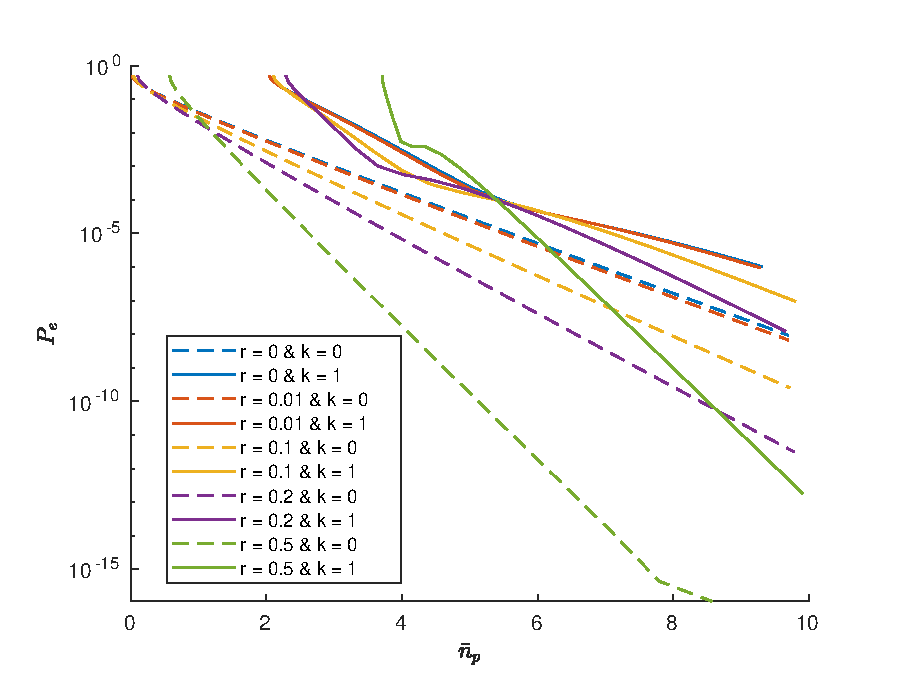
\includegraphics[width=0.8\textwidth]{fig3.7.eps}
                % This file was created by matlab2tikz.
%
%The latest updates can be retrieved from
%  http://www.mathworks.com/matlabcentral/fileexchange/22022-matlab2tikz-matlab2tikz
%where you can also make suggestions and rate matlab2tikz.
%
\definecolor{mycolor1}{rgb}{0.00000,0.44706,0.74118}%
\definecolor{mycolor2}{rgb}{0.85098,0.32549,0.09804}%
\definecolor{mycolor3}{rgb}{0.92941,0.69020,0.12941}%
\definecolor{mycolor4}{rgb}{0.49020,0.18039,0.56078}%
\definecolor{mycolor5}{rgb}{0.46667,0.67451,0.18824}%
%
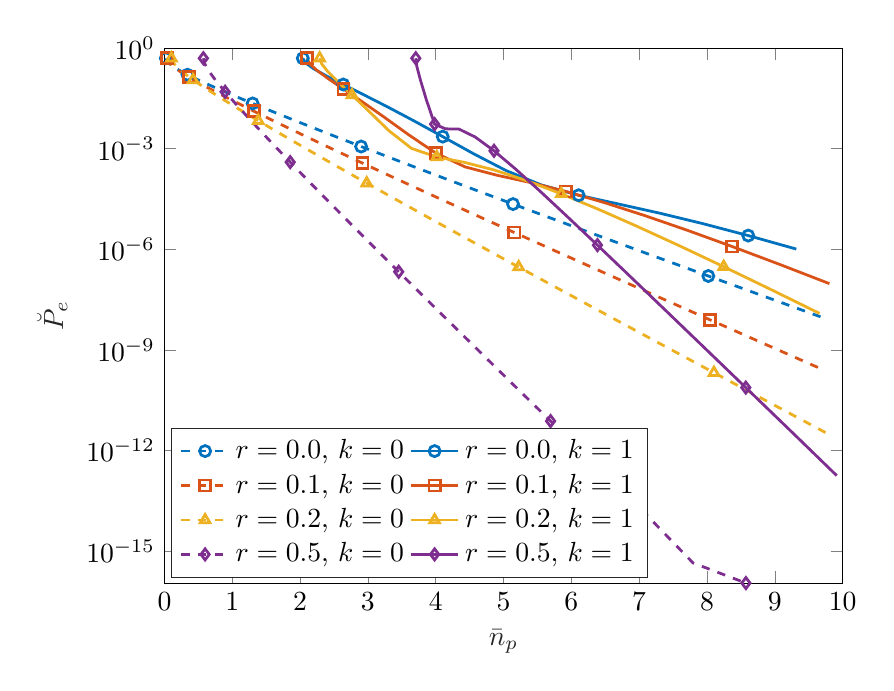
\begin{tikzpicture}

\begin{axis}[%
width=4.521in*0.75,
height=3.566in*0.75,
at={(0.758in,0.481in)},
scale only axis,
xmin=0,
xmax=10,
xlabel style={font=\color{white!15!black}},
xlabel={$\bar{n}_p$},
ymode=log,
ymin=1.11022302462516e-16,
ymax=1,
yminorticks=true,
ylabel style={font=\color{white!15!black}},
ylabel={$\breve{P}_e$},
axis background/.style={fill=white},
%axis x line*=bottom,
%axis y line*=left,
legend style={at={(0.01,0.01)}, anchor=south west, legend cell align=left, align=left, draw=white!15!black, legend columns=2}
]
\addplot [color=mycolor1, dashed, line width=1.0pt, mark=o, mark options={solid, mycolor1}, mark repeat={4}]
  table[row sep=crcr]{%
0.0200000000020406	0.5\\
0.0400000000020402	0.402886691283791\\
0.10000000000204	0.311248795396143\\
0.20000000000204	0.229705791588748\\
0.34000000000204	0.161367836859558\\
0.52000000000204	0.107527572164159\\
0.740000000002041	0.0677402706067528\\
1.00000000000204	0.040228893816313\\
1.30000000000204	0.0224701735043469\\
1.64000000000204	0.0117874985937501\\
2.02000000000204	0.00580411358757571\\
2.44000000000204	0.00268301603344689\\
2.90000000000204	0.00116504474732904\\
3.40000000000204	0.000475529564681332\\
3.94000000000204	0.00018252496091431\\
4.52000000000204	6.58942320924671e-05\\
5.14000000000204	2.2372962739603e-05\\
5.80000000000205	7.14262612222516e-06\\
6.50000000000204	2.14348977123358e-06\\
7.24000000000202	6.04459258424228e-07\\
8.02000000000186	1.60120172343348e-07\\
8.84000000000037	3.98308174776041e-08\\
9.69999999998796	9.30169952173543e-09\\
};
\addlegendentry{$r = 0.0$, $k = 0$}

\addplot [color=mycolor1, line width=1.0pt, mark=o, mark options={solid, mycolor1}, mark repeat={4}]
  table[row sep=crcr]{%
2.04000000000614	0.5\\
2.07980388157475	0.365238945696499\\
2.19695222552987	0.245075031520992\\
2.38527239346053	0.149666545304717\\
2.6362387582965	0.0824178394910576\\
2.94079284127565	0.0405450261122263\\
3.29080184759698	0.0176651515033895\\
3.67986533387235	0.0067767120762533\\
4.10351356897534	0.00229560228979309\\
4.55900917319244	0.000707434570884347\\
5.04497309453299	0.00021948919726017\\
5.56098876721283	8.28582489130203e-05\\
6.10726290808727	4.1022391904566e-05\\
6.68436781659824	2.27142595118912e-05\\
7.29306128054439	1.21004232845334e-05\\
7.93416896319587	5.8707409222869e-06\\
8.60851248045389	2.56977332785402e-06\\
9.31686877149291	1.01844033345566e-06\\
};
\addlegendentry{$r = 0.0$, $k = 1$}

\addplot [color=mycolor2, dashed, line width=1.0pt, mark=square, mark options={solid, mycolor2}, mark repeat={4}]
  table[row sep=crcr]{%
0.0404680907314567	0.5\\
0.0604680907314585	0.392901670542549\\
0.120468090731458	0.293128630573881\\
0.220468090731458	0.206620339442921\\
0.360468090731457	0.136941029534563\\
0.540468090731457	0.084941538631533\\
0.760468090731459	0.0491016108355734\\
1.02046809073146	0.026360899632598\\
1.32046809073146	0.0131130551179189\\
1.66046809073146	0.00603787611242568\\
2.04046809073146	0.00257369694341059\\
2.46046809073146	0.00101640450241469\\
2.92046809073146	0.000372205972558992\\
3.42046809073146	0.00012645461779881\\
3.96046809073146	3.98629468535416e-05\\
4.54046809073146	1.16575616797565e-05\\
5.16046809073146	3.16151968782208e-06\\
5.82046809073146	7.94771541634542e-07\\
6.52046809073146	1.85116668105501e-07\\
7.26046809073146	3.99314517562921e-08\\
8.04046809073146	7.97410959485489e-09\\
8.86046809073146	1.47367751335281e-09\\
9.72046809073146	2.51973775178271e-10\\
};
\addlegendentry{$r = 0.1$, $k = 0$}

\addplot [color=mycolor2, line width=1.0pt, mark=square, mark options={solid, mycolor2}, mark repeat={4}]
  table[row sep=crcr]{%
2.1016048937167	0.5\\
2.13722342176411	0.351557555027417\\
2.24231126096937	0.222160769918723\\
2.41204284470634	0.124222362453645\\
2.63974114418153	0.0603925042112791\\
2.91829336919182	0.0250484475022711\\
3.24129213294307	0.00872798119433771\\
3.60367379405264	0.00258598757293121\\
4.0018832937306	0.000741253402724129\\
4.43372687028477	0.000287093498001045\\
4.89808386454928	0.000162974574048513\\
5.39459822969919	9.8293093218349e-05\\
5.9234122263596	5.2962165794368e-05\\
6.48496287009384	2.48063685127087e-05\\
7.07983886502512	1.01844444848065e-05\\
7.70868661927138	3.70885692668743e-06\\
8.37215237665687	1.20946493997742e-06\\
9.07084922366429	3.55623495429391e-07\\
9.80534037124127	9.47534976036835e-08\\
};
\addlegendentry{$r = 0.1$, $k = 1$}

\addplot [color=mycolor3, dashed, line width=1.0pt, mark=triangle, mark options={solid, mycolor3}, mark repeat={4}]
  table[row sep=crcr]{%
0.102693819275224	0.5\\
0.122693819275224	0.381945077116474\\
0.182693819275225	0.273671210068553\\
0.282693819275225	0.18272455257\\
0.422693819275225	0.112952560216816\\
0.602693819275226	0.0642502792905548\\
0.822693819275224	0.03345396094764\\
1.08269381927522	0.0158838250522541\\
1.38269381927522	0.00686368066298626\\
1.72269381927522	0.00269897231763505\\
2.10269381927523	0.000966736234112642\\
2.52269381927523	0.000315777240763426\\
2.98269381927522	9.41232533182568e-05\\
3.48269381927522	2.56024275193667e-05\\
4.02269381927522	6.35315675889814e-06\\
4.60269381927523	1.43743867431212e-06\\
5.22269381927523	2.96354467355098e-07\\
5.88269381927523	5.5640574203597e-08\\
6.58269381927523	9.50809414534959e-09\\
7.32269381927523	1.47814516182621e-09\\
8.10269381927523	2.08976613791378e-10\\
8.92269381927523	2.68594035901515e-11\\
9.78269381927522	3.13798986795177e-12\\
};
\addlegendentry{$r = 0.2$, $k = 0$}

\addplot [color=mycolor3, line width=1.0pt, mark=triangle, mark options={solid, mycolor3}, mark repeat={4}]
  table[row sep=crcr]{%
2.28886800904409	0.5\\
2.31999800521609	0.335903697984307\\
2.41216418530892	0.196933331036258\\
2.56201679884254	0.0981076147304128\\
2.76489646890086	0.040185809256969\\
3.0158018679935	0.0130832203468926\\
3.31018324953374	0.00344887391962134\\
3.64440096753075	0.00101951363497232\\
4.01585991019939	0.000567040966715227\\
4.42292358106145	0.000392962039574174\\
4.86472316966757	0.000231481537813827\\
5.34094583218671	0.000111581978084918\\
5.85164780473884	4.51448958011524e-05\\
6.39710893432961	1.56946401249081e-05\\
6.97772869816361	4.76400489057838e-06\\
7.59395670680091	1.27574898745042e-06\\
8.24624906333657	3.03436716753147e-07\\
8.93504283030325	6.43988304904752e-08\\
9.66074253748888	1.2235391422255e-08\\
};
\addlegendentry{$r = 0.2$, $k = 1$}

\addplot [color=mycolor4, dashed, line width=1.0pt, mark=diamond, mark options={solid, mycolor4}, mark repeat={4}]
  table[row sep=crcr]{%
0.573942245572178	0.5\\
0.593942245028823	0.342499519674481\\
0.653942245170735	0.20790550335767\\
0.753942245341616	0.110057719920144\\
0.893942244583911	0.0500472584431716\\
1.07394224497389	0.0193143675146228\\
1.293942244546	0.00628332214973615\\
1.55394224371114	0.00172174882973891\\
1.85394224420503	0.000398395169961208\\
2.19394224278596	7.80046198984863e-05\\
2.57394224201761	1.29266966575337e-05\\
2.99394224220523	1.81130230003657e-06\\
3.45394223899107	2.14287482536157e-07\\
3.95394223844945	2.13728023612525e-08\\
4.49394223715584	1.79488168772224e-09\\
5.07394223021208	1.26788857190974e-10\\
5.693942230031	7.52714557350487e-12\\
6.35394222368679	3.74977826567147e-13\\
7.05394220748901	1.55431223447522e-14\\
7.79394220753813	4.44089209850063e-16\\
8.57394218450974	1.11022302462516e-16\\
9.39394214003978	0\\
};
\addlegendentry{$r = 0.5$, $k = 0$}

\addplot [color=mycolor4, line width=1.0pt, mark=diamond, mark options={solid, mycolor4}, mark repeat={4}]
  table[row sep=crcr]{%
3.7061308486222	0.5\\
3.72318775095693	0.276003723186423\\
3.77462452178882	0.111964236743116\\
3.86118165596315	0.0292098038693948\\
3.98392247081425	0.00541832505604978\\
4.14404207041508	0.00392337294658973\\
4.34269448841782	0.00386065139664005\\
4.58087300628471	0.00224591730584783\\
4.85935291484359	0.000870231139084243\\
5.17868537920139	0.000246879397142796\\
5.53922245734845	5.40728938508428e-05\\
5.94115678880561	9.42866109115981e-06\\
6.38456317979691	1.33219265713302e-06\\
6.86943477192184	1.54061789436888e-07\\
7.39571266351863	1.46675764867155e-08\\
7.96330772743687	1.15372272846415e-09\\
8.57211535637269	7.51390061282109e-11\\
9.22202638435226	4.05170341721828e-12\\
9.9129334474046	1.78523862359725e-13\\
};
\addlegendentry{$r = 0.5$, $k = 1$}
\end{axis}
\end{tikzpicture}%
                \caption{MDEP of noisy PASS quantum BPSK system as function of $\bar{n}_p$ with
                $N=40$, $\bar{n}=10^{-2}$, $\theta=\pi$ and $p_0=p_1=1/2$.}
                \label{fig:3.7}
            \end{center}
        \end{figure}